\documentclass[11pt,titlepage]{article}
\usepackage[a4paper,
            left=3cm,
            right=3cm,
            top=2cm,
            bottom=2cm]{geometry}
\usepackage[spanish]{babel}
\usepackage[none]{hyphenat}
\usepackage[utf8]{inputenc}
\usepackage[titletoc]{appendix}
\usepackage{csquotes}

\usepackage{amsmath,mathtools,cancel,multicol}
\usepackage{graphicx,booktabs,tabularx,amssymb,amsfonts}
\graphicspath{{./media/}}
\usepackage[shortlabels]{enumitem}
\usepackage{pdfpages}

\usepackage{verbatim}

\usepackage{tcolorbox}
\newtcolorbox{commBoxy}{
	colback=red!5!white,
	colframe=red!75!black}
\newtcolorbox{titleBoxy}[1]{
	colback=red!5!white,
	colframe=red!75!black,
	fonttitle=\mdseries,
	title=#1}

\usepackage[pdfauthor={Alejandro Nahuel Heir},
            colorlinks,
			linkcolor=red]{hyperref}

%Custom Commands:
\newcommand{\commLim}[2]{\lim_{#1 \to #2}}
\newcommand{\displayLim}[2]{\displaystyle \commLim{#1}{#2}}

\newcommand{\littleTitle}[1]{
	\noindent \ignorespaces
	\small \textbf{#1} \normalsize
	\ignorespaces \ignorespacesafterend
}

\newcommand{\comillas}[1]{``#1''}

\DeclareMathOperator{\arcsinh}{arcsinh}
\DeclareMathOperator{\arccosh}{arccosh}
\DeclareMathOperator{\arctanh}{arctanh}

\begin{document}

\begin{titlepage}
	\centering
	{\Large Instituto Tecnológico Buenos Aires \par}
	\vspace{2cm}
	{\huge Matemática I - 93.17 \par}
	\vspace{2cm}
	{\Huge Resumen Práctico \par}
	\vspace{2cm}
	{\ttfamily Alejandro Nahuel Heir \par}
	{\ttfamily \href{mailto:aheir@itba.edu.ar}{aheir@itba.edu.ar} \par}
	\vspace{0.5cm}
	{\ttfamily 2021 \par}
\end{titlepage}

\begin{abstract}
	Usar el presente material a modo de refuerzo y/o repaso de los contenidos; no contiene ninguna justificación 
	teórica profunda. Fue realizado principalmente a modo de práctica para con \LaTeX. Cualquier sugerencia, correción
	y/o similar, \href{mailto:aheir@itba.edu.ar}{es bienvenida}.
\end{abstract}

\tableofcontents
\newpage
\listoffigures
\newpage
\listoftables
%\setcounter{tocdepth}{4}
%\setcounter{secnumdepth}{4}
%\setcounter{tocdepth}{5}
%\setcounter{secnumdepth}{5}
\newpage

\part{Primer Parcial}
\section{Límites}

\subsection{Cambio de variable}
Sean $\lim_{y \to b} g(y)=L, \lim_{x \to a} f(x)=b, f(x) \neq b \text{ en un entorno reducido de } a$,\\
entonces
\begin{equation}\label{cambiovar}
	\lim_{x \to a} g(f(x)) = \lim_{y \to b} g(y) = L
\end{equation}

\subsection{Cero por acotada}
Sean $\lim_{x \to a} g(x) = 0, \nexists \lim_{x \to a} f(x) \text{, con \textit{f} acotada en un entorno reducido de \textit{a}}$,\\
entonces
\begin{equation}\label{ceroacotada}
		\lim_{x \to a} \overbrace{f(x)}^{acotada} \cancelto{0}{g(x)} = 0
\end{equation}

\subsection{Lema del Sandwich}
Sean $f(x) \leq g(x) \leq h(x), \forall x \in E^{\ast}_{(a,r)} \text{con } r>0.$
Si $\lim_{x \to a} f(x) = \lim_{x \to a} h(x) = L$, entonces
\begin{equation}\label{sandwich}
	\lim_{x \to a} g(x) = L
\end{equation}

\littleTitle{Observación}\par
Sea $\lim_{x \to a} |f(x)| = 0$, y sabiendo que $-|f(x)| \leq f(x) \leq |f(x)|$, se deduce por Lema del Sandwich que
\begin{equation}
	\lim_{x \to a} |f(x)| = 0 \Rightarrow \lim_{x \to a} f(x) = 0
\end{equation}

\subsection{Sobre límites laterales}
\begin{equation*}
	\nexists \lim_{x \to a} f(x) \text{ si }
	\begin{cases}
		\lim_{x \to a^{+}} f(x) = L_1 \\
		\lim_{x \to a^{-}} f(x) = L_2
	\end{cases}
	L_1 \neq L_2
\end{equation*}
\begin{equation*}
	\nexists \lim_{x \to a} f(x) \text{ si }
	\begin{cases}
		\commLim{x}{a^{+}} f(x) = L \\
		\nexists \commLim{x}{a^{-}} f(x)
	\end{cases}
\end{equation*}
\vspace{0.5cm}
\begin{equation}
	\therefore \commLim{x}{a} f(x) = L \Leftrightarrow \commLim{x}{a^{+}} f(x) = \commLim{x}{a^{-}} f(x) = L
\end{equation}

\subsection{Límites importantes}
\subsubsection{Trigonométricos}
\begin{multicols}{3}
	\begin{enumerate}[label=\alph*.]
		\item $ \displayLim{x}{0} \dfrac{\sin x}{x} = 1 $
		\item $ \displayLim{x}{0} \frac{x}{\sin x} = 1 $
		      %\item $ \displayLim{x}{0} \frac{\cos x}{x} = \infty $
		\item $ \displayLim{x}{0} \frac{\tan x}{x} = 1 $
		\item $ \displayLim{x}{0} \frac{x}{\tan x} = 1 $
		\item $ \displayLim{x}{0} \frac{\arctan x}{x} = 1 $
	\end{enumerate}
\end{multicols}

\subsubsection{Relativos a \textit{e}}
\littleTitle{Igualdad importante}\par
	\begin{equation}
		\boldsymbol{f(x)^{g(x)} = e^{g(x) \ln(f(x))}}
	\end{equation}

\begin{enumerate}[label=\alph*.]
	\item $ \displayLim{x}{a} \left(1+\frac{1}{f(x)}\right)^{f(x)} = e, \quad	\text{si} \commLim{x}{a} f(x) = \infty $
	\item $ \displayLim{x}{a} (1+f(x))^{\frac{1}{f(x)}} = e, \quad	\text{si} \commLim{x}{a} f(x) = 0 $
	\item $ \displayLim{x}{a} \frac{\ln(1 + f(x))}{f(x)} = 1, \quad	\text{si} \commLim{x}{a} f(x) = 0 $
	\item $ \displayLim{x}{a} \frac{e^{f(x)}-1}{f(x)} = 1, \quad \text{si} \commLim{x}{a} f(x) = 0 $
\end{enumerate}

\subsection{Sobre límites infinitos}
\begin{multicols}{2}
	\begin{enumerate}[label=\alph*.]
		\item $ \displayLim{x}{0} \frac{k}{x} = \infty$, \quad con $ k \in \mathbb{R} - \left\{0 \right\} $
		\item $ \displayLim{x}{\infty} \frac{k}{x} = 0$, \quad con $ k \in \mathbb{R} $
		\item $ \displayLim{x}{\infty} kx = \infty$, \quad con $k \in \mathbb{R} - \left\{0\right\} $
		\item $ \displayLim{x}{\infty} k + x = \infty$, \quad con $ k \in \mathbb{R} $
	\end{enumerate}
\end{multicols}

\vspace{1cm}
\section{Continuidad}
\subsection{Definición}
$f$ es continua en $a \in \mathbb{R}$ si:
\begin{itemize}
	\item $a \in Dom(f)$
	\item $\exists \commLim{x}{a} f(x)$
	\item $\commLim{x}{a} f(x) = f(a)$
\end{itemize}

\subsection{Propiedades}
Sean $f$ y $g$ continuas en $a \in \mathbb{R}$:
\begin{multicols}{2}
	\begin{itemize}
		\item $cf$ es continua en $a$, $\forall c \in \mathbb{R}$
		\item $f \pm g$ es continua en $a$
		\item $fg$ es continua en a
		\item $\dfrac{f}{g}$ es continua en $a$, si $g(a) \neq 0$
	\end{itemize}
\end{multicols}
	
\subsection{Funciones continuas en todo su dominio}
\begin{multicols}{2}
	\begin{itemize}
		\item Polinómicas
		\item Trigonométricas (directas o inversas)
		\item Exponenciales
		\item Logarítmicas
		\item Raíces (excepto $\sqrt[n]{x}$ en $x = 0$ para $n$ pares)
	\end{itemize}
\end{multicols}

\subsection{Composición}
Si $f$ es continua en $x=a$, y $g(z)$ es continua en $z=f(a)$, entonces $h(x) = (g\circ f)(x)$ es continua en $a$.

\subsection{Discontinuidades}
$f$ es discontinua en $a \in \mathbb{R}$ si se cumple \underline{\emph{al menos una}} de las siguientes condiciones:
\begin{itemize}
	\item $a \notin Dom(f)$
	\item $\nexists \commLim{x}{a} f(x)$ 
	\item $\commLim{x}{a} f(x) \neq f(a)$ 
\end{itemize}

\subsubsection{Evitables}
$a \in \mathbb{R}$ es discontinuidad evitable si se cumple simultáneamente
\begin{multicols}{3}
	\begin{itemize}
		\item $f(a) = L_1 \in \mathbb{R}$
		\item $\exists \displayLim{x}{a} f(x) = L_2 \in \mathbb{R}$
		\item $L_1 \neq L_2 \neq \infty$
	\end{itemize}
\end{multicols}
\emph{Si se redefine $f(x)$ en $x = a$ como $f(a) = L_2$, $f$ pasa a ser continua en $a$.}

\subsubsection{No evitables o esenciales}

\littleTitle{Tipo salto}\par
$a \in \mathbb{R}$ es discontinuidad esencial tipo salto si
\begin{equation*}
	\commLim{x}{a^{-}} f(x) = L_1 \neq \commLim{x}{a^{+}} f(x) = L_2, \quad L_1, L_2 \in \mathbb{R}
\end{equation*}

\littleTitle{Tipo asíntota (vertical)}\par
$a \in \mathbb{R}$ es discontinuidad esencial tipo asíntota si se cumple \underline{\emph{alguna}} de las siguientes igualdades
\begin{equation*}
	\commLim{x}{a^{-}} f(x) = \infty \qquad \text{o} \qquad \commLim{x}{a^{+}} f(x) = \infty
\end{equation*}

\littleTitle{\comillas{De otro tipo}}\par
$a \in \mathbb{R}$ es discontinuidad esencial de otro tipo si no es ninguna de las anteriores. Por ejemplo, $a = 0, f(a), \text{ con } f(x) = \sin \dfrac{1}{x}$
\begin{figure}[htb!]
	\centering 
	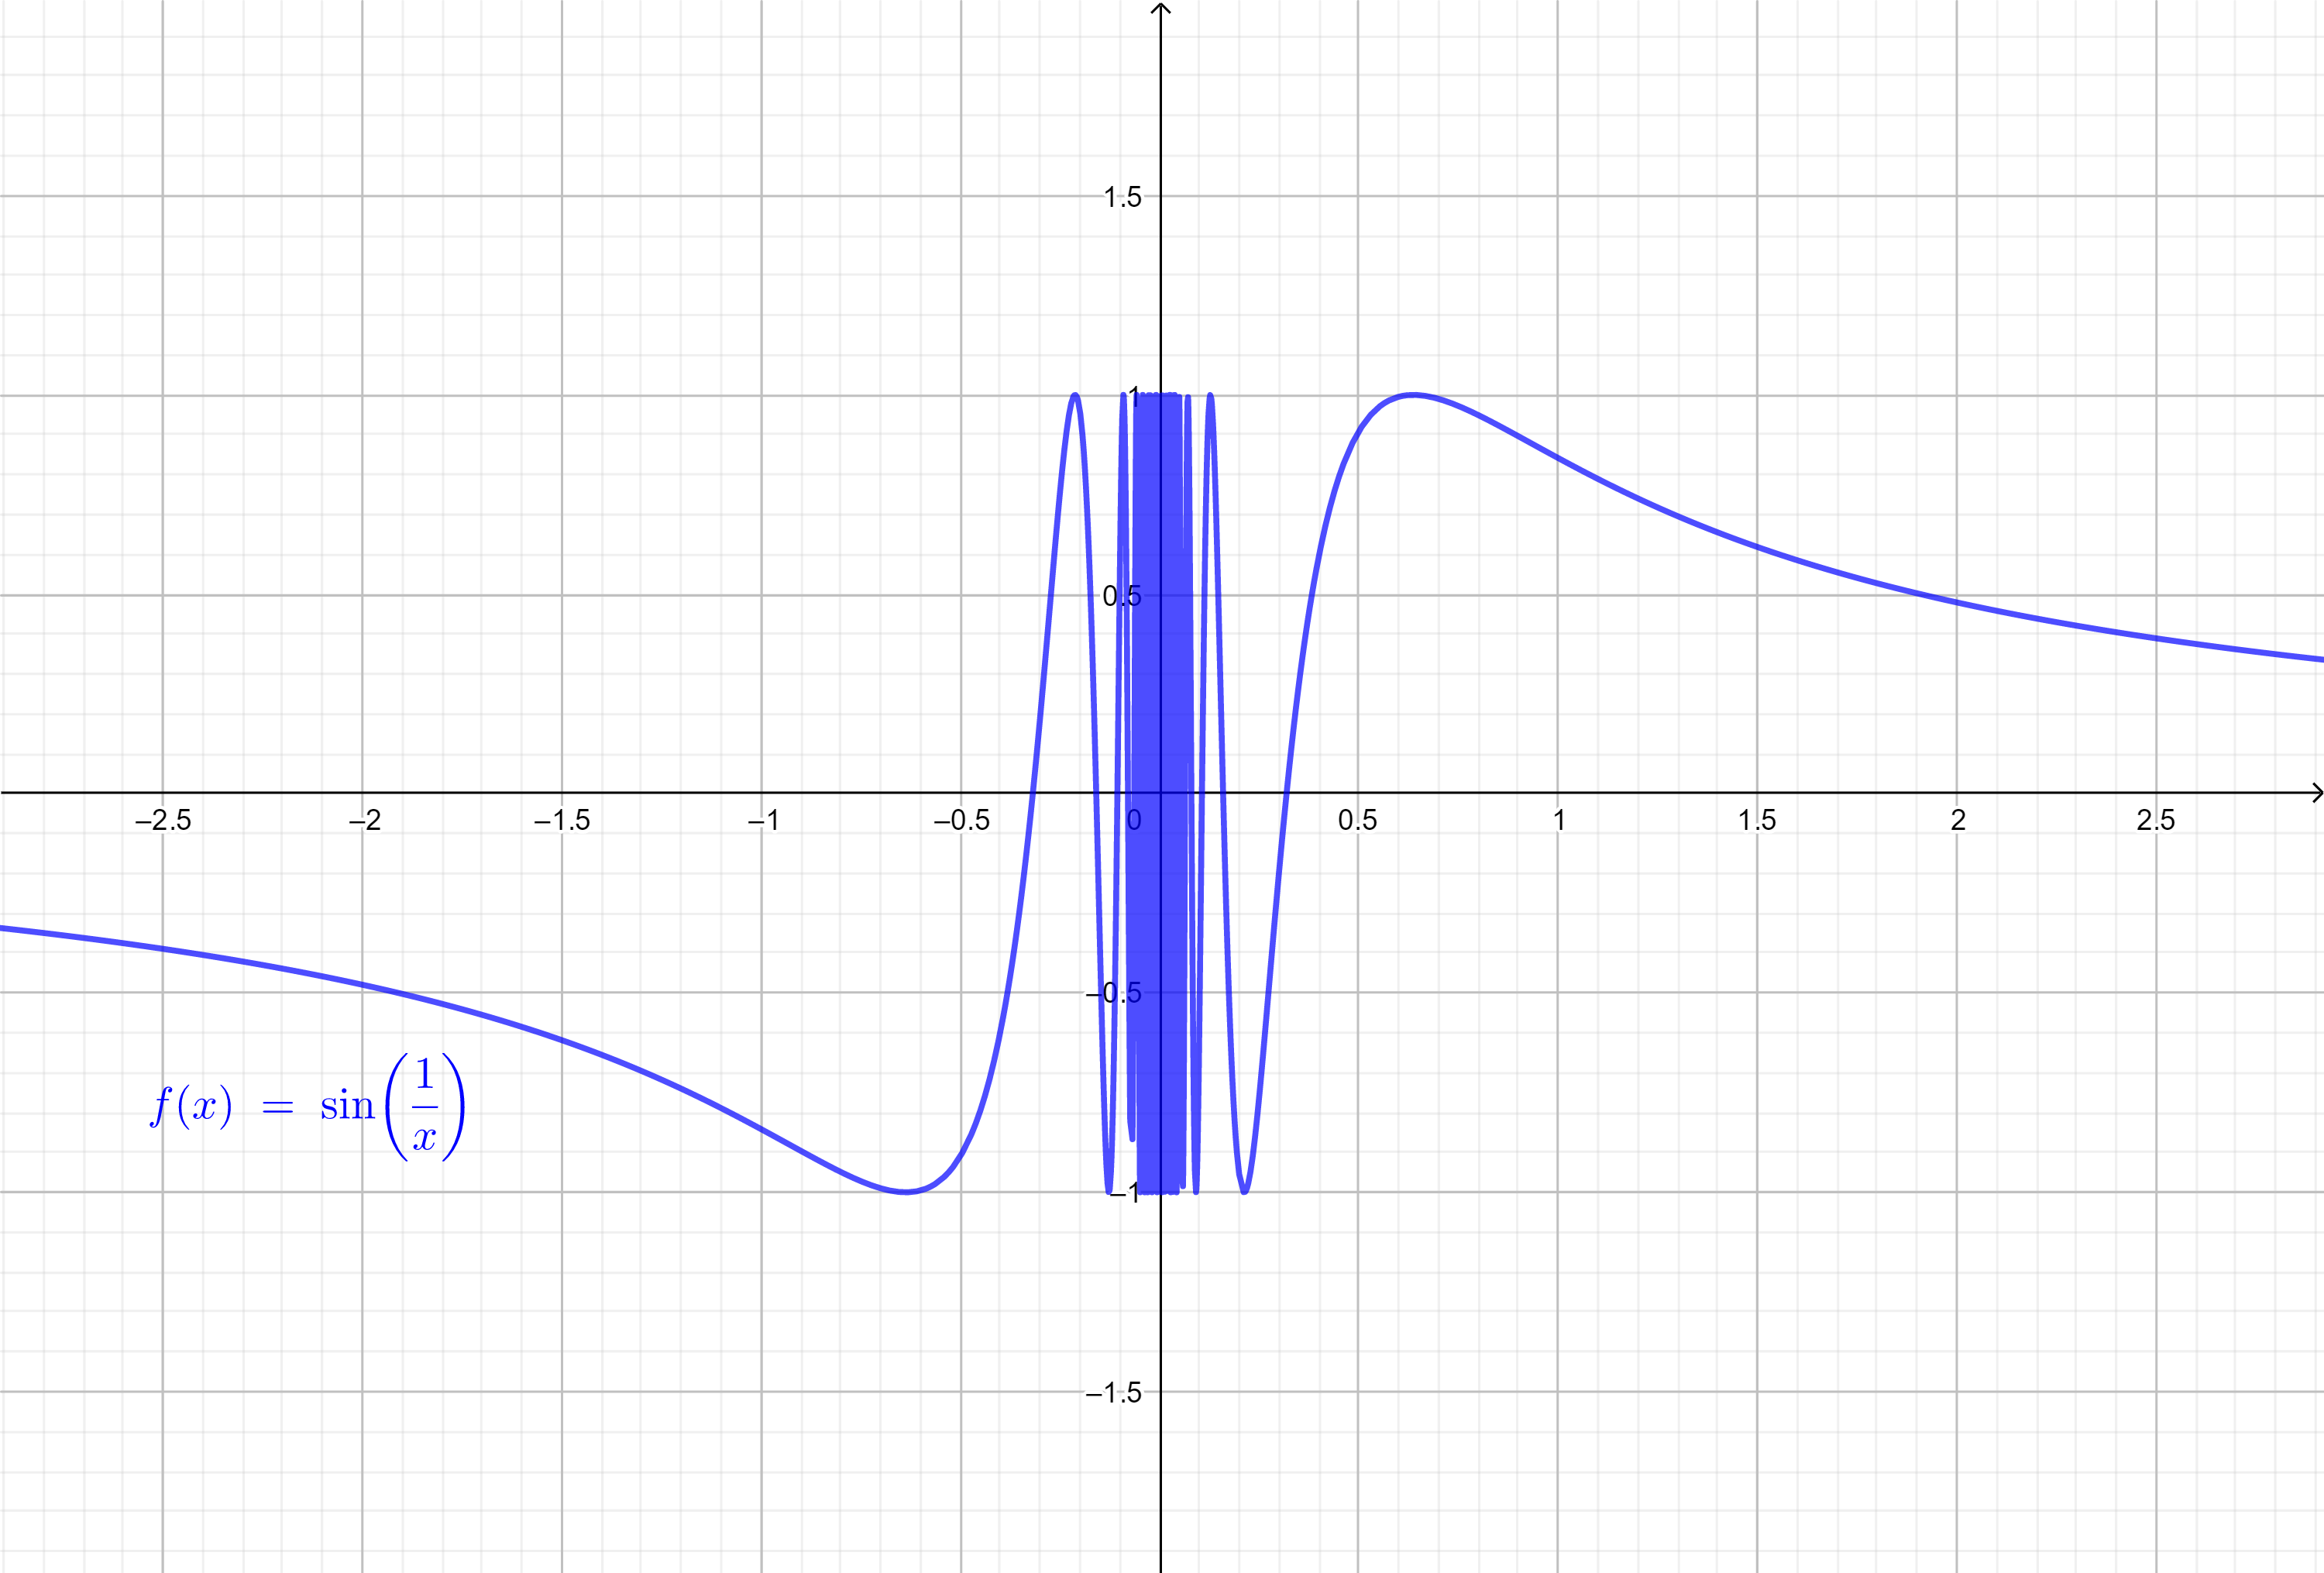
\includegraphics[scale=1.5]{discontinuidad_otro_tipo.png}
	\caption{Gráfico de la función $\sin \dfrac{1}{x}$}
	\label{fig:discontinuidad_otro_tipo}
\end{figure}

\pagebreak

\subsection{Teorema de Bolzano - T.B.}
\begin{commBoxy}
	Si $f$ es continua en $[a,b]$, y $f(a)f(b) < 0$ (\emph{tienen signos opuestos}), entonces 
	\begin{equation}
		\boldsymbol{\exists c \in \left(a,b\right) / f(c) = 0} \text{ (\emph{al menos una raiz})}
	\end{equation}
\end{commBoxy}
Si $f$ es continua en un intervalo abierto $\left(a,b\right)$, se debe cumplir que $\commLim{x}{a^{+}} f(x) = f(a)$, y que $\commLim{x}{b^{-}} f(x) = f(b).$

\subsubsection{Uso}
\littleTitle{Hallar raíces mínimas de una función}\par
Dada una $f(x)$ igualada a $0$, continua en un intervalo dado, hallar por tanteo dos valores de $x$ (que pertenezcan 
al intervalo donde $f$ es continua) para los cuales $f(x)$ tenga \emph{distinto signo}. Luego, por \emph{T.B.}, esa 
función tendrá \emph{al menos} una raíz entre esos dos valores de $x$ elegidos.\par
Cabe resaltar que esto puede emplearse también para conocer soluciones mínimas de una ecuación igualada a $0$.

\subsection{Corolario del Teorema de Bolzano - C.T.B.}
\begin{commBoxy}
	Sea $f$ continua en $(a,b)$, con $f(x) \neq 0 \ \forall x \in (a,b)$, entonces $f$ mantiene su signo en $(a,b)$. Es decir:
	\begin{equation}
		\boldsymbol{f(x) > 0 \ \forall x \in (a,b) \qquad \text{ó} \qquad f(x) < 0 \ \forall x \in (a,b)} 
	\end{equation}
\end{commBoxy}

\subsubsection{Uso}
\littleTitle{Hallar conjuntos de positividad y negatividad de una función}\par
Dada una función, y conociendo su dominio y conjunto de ceros, se puede \comillas{partir} el dominio de la función en intervalos donde la misma es
continua y no nula (esto último sabiendo el conjunto de ceros). A lo largo de cada intervalo, si la función es continua en él, mantendrá 
su signo; basta tomar una $x$ cualquiera en ese intervalo y evaluarla en la función para saber el signo en todo ese intervalo.

\subsection{Teorema del Valor Intermedio - T.V.I.}
Sea $f$ continua en $[a,b]$, $f(a) = c, \ f(b) = d, \ c \neq d,$ entonces:
\begin{enumerate}[label=\alph*.]
	\item $c < d \Rightarrow [c,d] \subset f\left([a,b]\right)$
	\item $d < c \Rightarrow [d,c] \subset f\left([a,b]\right)$
\end{enumerate}

\littleTitle{Generalización}\par
Sea $f$ continua en (a,b), $\commLim{x}{a^{+}} f(x) = c, \ \commLim{x}{b^{-}} f(x) = d$, entonces:
\begin{enumerate}[label=\alph*.]
	\item $c < d \Rightarrow [c,d] \subset f\left([a,b]\right)$
	\item $d < c \Rightarrow [d,c] \subset f\left([a,b]\right)$
\end{enumerate}

\pagebreak

\subsection{Teorema para evaluar sobreyectividad}
Sea $f$ continua en $(a,b)$, donde $a$ podría ser $-\infty$ y $b$ $+\infty$. Si
\begin{equation*}
	\commLim{x}{a^{+}} f(x) = -\infty \quad \wedge \quad \displayLim{x}{b^{-}} f(x) = +\infty \\
\end{equation*}
\begin{center}
\Large{\emph{o}}
\end{center}
\begin{equation*}
	\commLim{x}{a^{+}} f(x) = +\infty \quad \wedge \quad \displayLim{x}{b^{-}} f(x) = -\infty \\
\end{equation*}
entonces
\begin{equation*}
	f\left((a,b)\right) = \mathbb{R}, \ \therefore \ f \ \text{\emph{es sobreyectiva}}
\end{equation*}

\vspace{1cm}
\section{Derivadas}

\subsection{Ecuaciones de rectas}
Sea $x_0 \in \mathbb{R}$ el punto en el cual la recta es tangente o normal a la función $f$.
\subsubsection{Recta tangente}
\begin{equation}
	r_{T}(x) = f(x_0) + f'(x_0)(x - x_0)
\end{equation}
\subsubsection{Recta normal}
\begin{equation}
	r_{N}(x) = f(x_0) + \left(\frac{-1}{f'(x_0)}\right)(x - x_0)
\end{equation}

\subsection{Derivada por definición}
La derivada de $f$ en $x_0$ es, si existe, el valor del límite del siguiente cociente incremental:
\begin{equation}
	\begin{aligned}
		f'(x_0) = \commLim{x}{x_0} \frac{\Delta f}{\Delta x} &= \commLim{x}{x_0} \frac{f(x) - f(x_0)}{x - x_0} \\ \\
		&= \commLim{h}{0} \frac{f(x_{0} + h) - f(x_0)}{h}
	\end{aligned}
\end{equation}

\subsection{Teorema en relación a la continuidad}
\begin{itemize}
	\item Si $\exists f'(x_0) \Rightarrow f$ es continua en $x_0$
	\item Si $f$ es discontinua en $x_0 \Rightarrow \nexists f'(x_0)$
\end{itemize}
\emph{$f$ continua en $x_0$ NO necesariamente implica $\exists f'(x_0)$.} Por ejemplo:
\begin{gather*}
	f(x) = |x| \text{ es continua en } \mathbb{R} \\ \\
	\commLim{x}{0} \frac{|x| - 0}{x} = \commLim{x}{0} sg(x), \quad \text{pero} \quad \nexists \commLim{x}{0} sg(x) \\ \\
	\therefore |x| \ \text{NO es derivable en} \ x_0 = 0
\end{gather*}

\subsection{Reglas de derivación}
Sean $f$ y $g$ derivables en $x_0 \in \mathbb{R}$:
\begin{itemize}
	\item[1.] $(cf)'(x_0) = cf'(x_0), \quad \forall c \in \mathbb{R}$
	\item[2.] $(f \pm g)'(x_0) = f'(x_0) \pm g'(x_0)$ 
	\item[3.] $(fg)' = f'(x_0)g(x_0) + f(x_0)g'(x_0)$
	\item[4.] $\left(\dfrac{f}{g}\right)' = \dfrac{f'(x_0)g(x_0) - f(x_0)g'(x_0)}{g^{2}(x_0)}, \quad g(x_0) \neq 0$
\end{itemize}

\subsection{Regla de la cadena}
Sea $f(x)$ derivable en $x_0$, y $g(y)$ derivable en $y_0$, entonces $h(x) = (g \circ f)(x)$ es derivable en $x_0$, y:
\begin{equation}
	h'(x_0) = (g \circ f)'(x) = g'\left(f(x_0)\right) \cdot f'(x_0)
\end{equation}

\subsection{Derivadas notables}
\begin{table}[h!]
	\centering
	\setlength{\tabcolsep}{10pt} % Default value: 6pt
	\renewcommand{\arraystretch}{2.5} % Default value: 1
	\begin{tabularx}{\textwidth}{lX||lX}
		\toprule
		$f(x)$            & $f'(x)$                                  & $f(x)$       & $f'(x)$                                          \\
		\midrule
		$c\in \mathbb{R}$ & 0                                        & $\cosh x$    & $\sinh x$                                        \\
		$x$               & 1                                        & $\sinh x$    & $\cosh x$                                        \\
		$a^{x}$           & $\ln(a)a^{x}, \quad a>0$                 & $\tanh x$    & $\dfrac{1}{\cosh^2 x}$                           \\
		$\ln x$           & $\dfrac{1}{x}$                           & $\arcsin x$  & $\dfrac{1}{\sqrt{1-x^2}}, \quad x\in (-1,1)$     \\
		$\log_{a} x$      & $\dfrac{1}{x\ln a}$                      & $\arccos x$  & $\dfrac{-1}{\sqrt{1-x^2}}, \quad x\in (-1,1)$    \\
		$|x|$             & $sg(x), \quad x \neq 0$                  & $\arctan x$  & $\dfrac{1}{1+x^2}, \quad x\in \mathbb{R}$        \\
		$x^{n}$           & $nx^{n-1}, \quad x>0, \ n\in \mathbb{R}$ & $\arcsinh x$ & $\dfrac{1}{\sqrt{1+x^2}}, \quad x\in \mathbb{R}$ \\
		$\sin x$          & $\cos x$                                 & $\arccosh x$ & $\dfrac{1}{\sqrt{x^2 -1}}, \quad x>1$            \\
		$\cos x$          & $\sin x$                                 & $\arctanh x$ & $\dfrac{1}{x^2 -1}, \quad x\in (-1,1)$           \\
		$\tan x$          & $\dfrac{1}{\cos ^{2}x}$                  &              &                                                  \\
		\bottomrule
	\end{tabularx}
	\caption{Derivadas notables}
\end{table}

\subsection{Sobre funciones partidas}
Siempre se debe analizar por definición la continuidad y derivabilidad en los valores de $x$ donde la función se parte.

\subsection{Teorema de la Función Inversa}
Sea $f: \ (a,b) \to \mathbb{R}$ continua e \emph{inyectiva}, entonces:
\begin{itemize}
	\item[1°] $Im(f)$ es un intervalo $(c,d)$, y $\exists f^{-1}: (c,d) \to (a,b)$, la cual es continua.
	\item[2°] Si $f$ es derivable en $x_0 \in (a,b)$, y $f'(x_0) \neq 0$, entonces $f'$ es derivable en $y_0 = f(x_0)$, y  
\end{itemize}
\begin{equation}
	\left(f^{-1}\right)'(y_0) = \frac{1}{f'(x_0)} = \frac{1}{f'\left(f^{-1}(y_0)\right)}
\end{equation}

\subsection{Aproximación lineal de un función}
\begin{equation}
	\begin{aligned}
		L(x) &= f(x_0) + f'(x_0)(x - x_0), \qquad \text{aproximación lineal de $f$ en $x_0$} \\ \\
		f(x) &\simeq L(x) \text{ cuando } x - x_0 \ll 1
	\end{aligned}
\end{equation}

\subsection{Aproximación diferencial de una función}
\begin{equation}
	\begin{aligned}
		df &= f'(x_0) \cdot \Delta x, \qquad \text{diferencial de $f$ en $x_0$} \\ \\
		\Delta f &\simeq df \text{ cuando } \Delta x \ll 1
	\end{aligned}
\end{equation}

\vspace{1.5cm}
\section{Teorema del Valor Medio}

\subsection{Teorema del Valor Intermedio - T.V.I.}
Sea $f$ continua en $[a,b]$, $f(a) = c$, $f(b) = d$, $c \neq d$:
\begin{itemize}
	\item[a.] $c < d \Rightarrow [c,d] \subset f\left([a,b]\right)$
	\item[b.] $d < c \Rightarrow [d,c] \subset f\left([a,b]\right)$
\end{itemize}
\littleTitle{Generalización}\par
Sea $f$ continua en (a,b), $\commLim{x}{a^{+}} f(x) = c \neq \commLim{x}{b^{-}} f(x) = d$, entonces:
\begin{itemize}
	\item[a.] $c < d \Rightarrow [c,d] \subset f\left([a,b]\right)$
	\item[b.] $d < c \Rightarrow [d,c] \subset f\left([a,b]\right)$
\end{itemize}

\subsection{Teorema de Fermat}
Sea $f: (a,b) \to \mathbb{R} / f$ alcanza un extremo en un $x_0 \in (a,b)$, entonces
\begin{gather}
	\nexists f'(x_0) \qquad \text{ó} \qquad f'(x_0) = 0
\end{gather}

\subsection{Teorema de Weierstrass - T.W.}
\begin{commBoxy}
	Sea $f: [a,b] \to \mathbb{R}$ continua, \emph{entonces} $f$ alcanza un $M$ (máximo) y $m$ (mínimo) en $[a,b]$.
	Además, por \emph{T.V.I.}:
	\begin{gather*}
		Im(f) = [m,M] \\ \\
		m \leq f(x) \leq M, \ \forall x \in [a,b] \\ \\
		\text{Si } m = M \Rightarrow f(x) \text{ es \emph{constante} en } [a,b]
	\end{gather*}
\end{commBoxy}

\subsection{Teorema de Rolle - T.R.}
\begin{commBoxy}
	\littleTitle{Hipótesis}\par
	\begin{itemize}
		\item $f: [a,b] \to \mathbb{R}$ continua; derivable en $(a,b)$.
		\item $\boldsymbol{f(a) = f(b)}$
	\end{itemize}
	
	\littleTitle{Tesis}
	\begin{gather}
		\exists c \in (a,b) / f'(c) = 0, \qquad \text{se afirma al menos unas raiz de $f'$}
	\end{gather}
\end{commBoxy}



\newpage
\part{Segundo Parcial}


\appendix
\begin{appendices}
	\section{Trigonometría 1}
	\clearpage
	%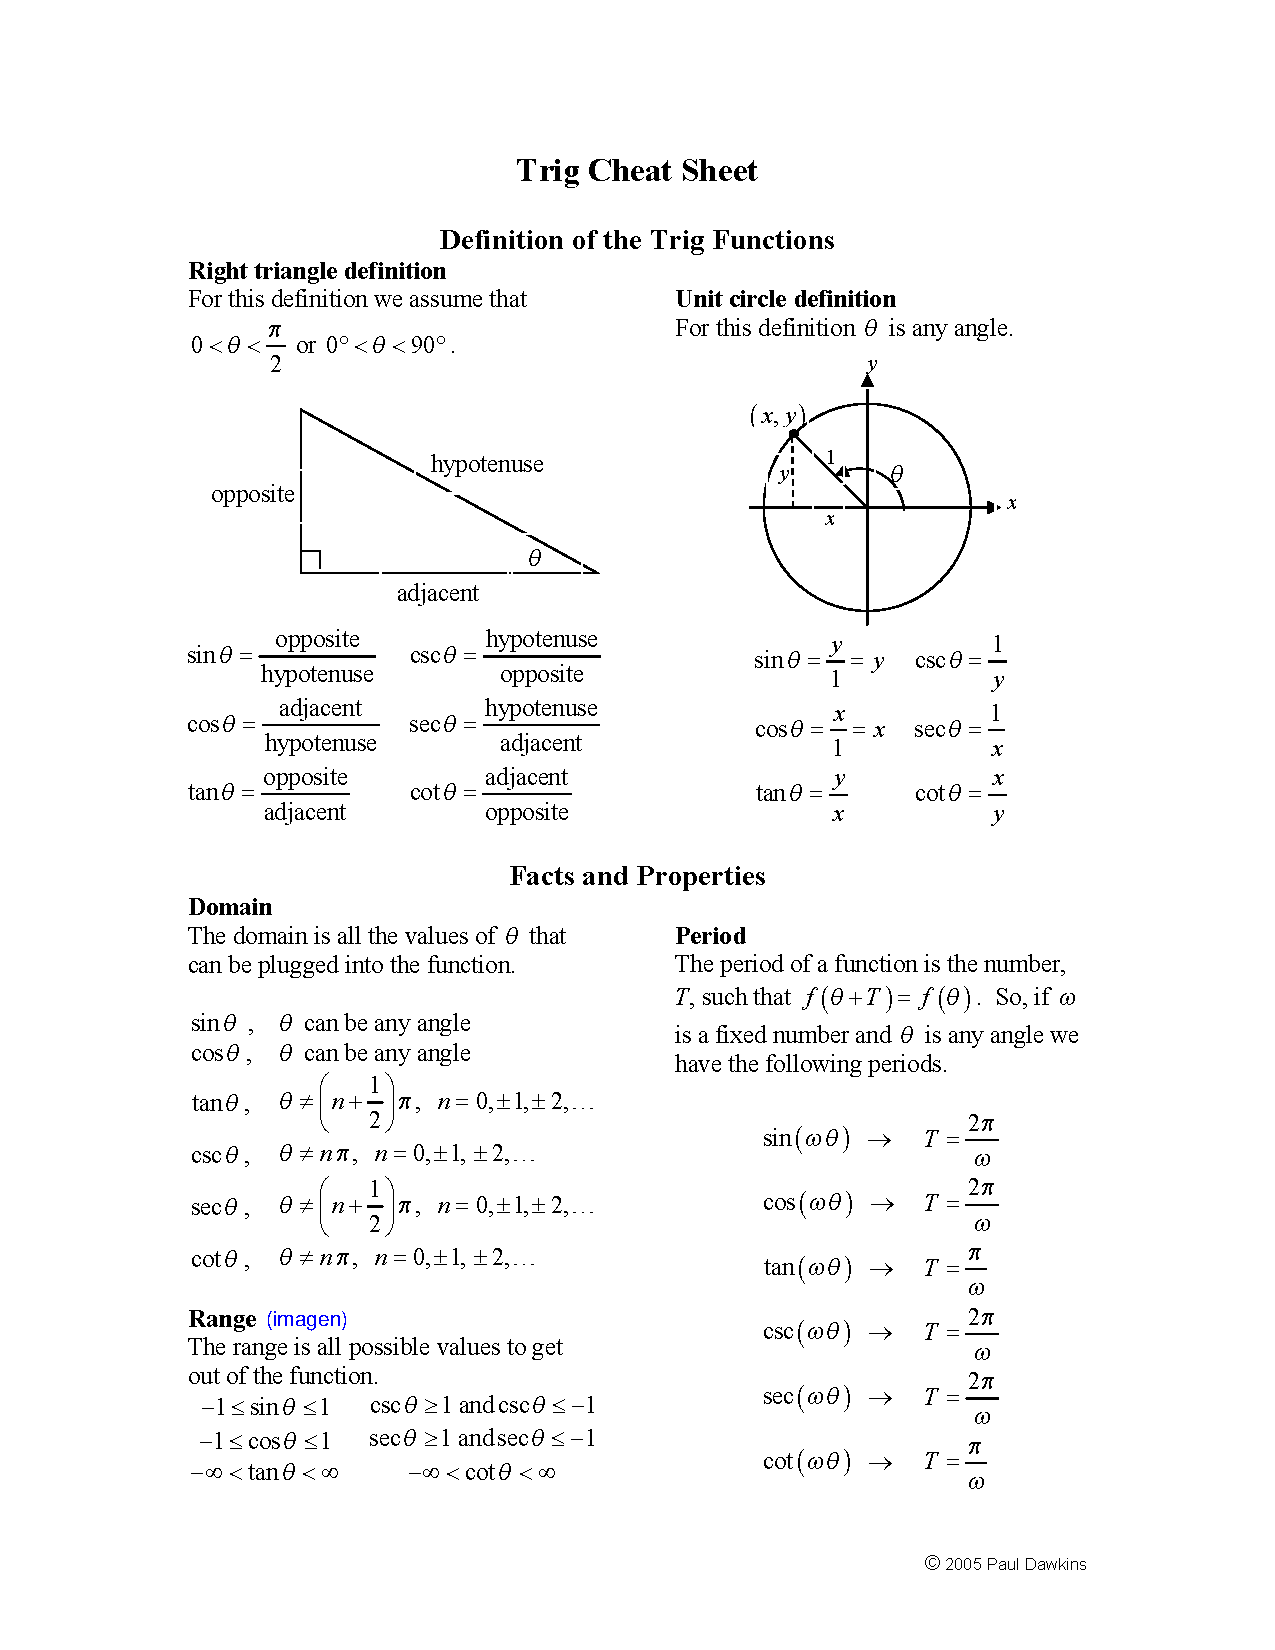
\includepdf[pages=-]{Trig_Cheat_Sheet.pdf}
	\section{Trigonometría 2}
	\clearpage
	%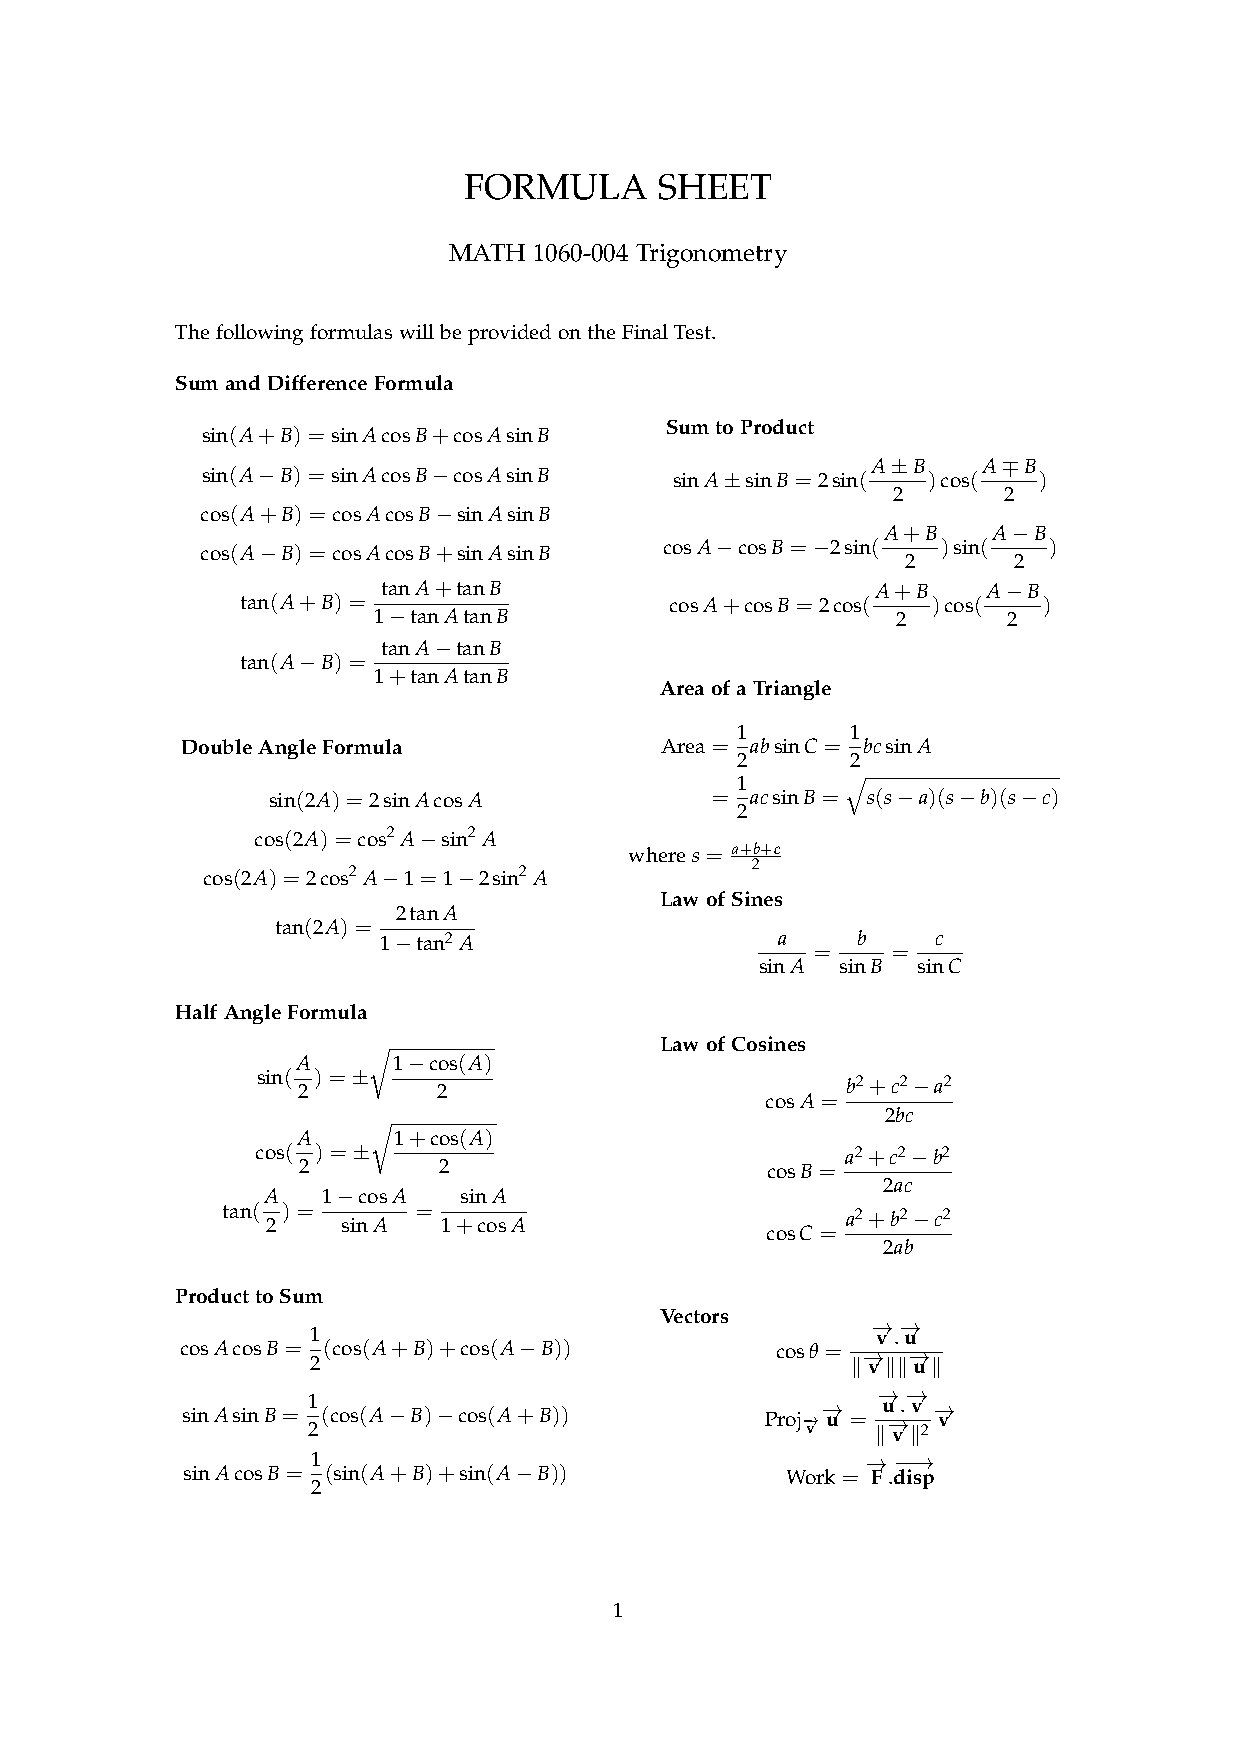
\includepdf[pages=-]{FormulaSheet.pdf}
\end{appendices}


\end{document}

